%%%%%%%%%%%%%%%%%%%%%%%%%%%%%%%%%%%%%%%%%%%%%%%%%%%%%%%%%%%%%%%%%%%%%%
%
%         Copyright (c) 2023, gitlabci_gallery / latex
%         All rights reserved.
%
%%%%%%%%%%%%%%%%%%%%%%%%%%%%%%%%%%%%%%%%%%%%%%%%%%%%%%%%%%%%%%%%%%%%%%

\documentclass[A4,svgnames,9pt,aspectratio=169]{beamer}
%% document options:
%% - aspectratio = { 43, 169, 1610 }
%% - utf8
%%


\setlength{\footskip}{300pt}
\usepackage[french]{babel}

\hypersetup{
   allcolors   = rouge_inria,
   pdfauthor   = {Duzés Florian},
   pdftitle    = {\@title},
   pdfsubject  = {Point hebdomadaire, bi-mensuel du stage},
   pdfkeywords = {entretien, observation du travail}
}

%%%%%%%%%%%%%%%%%%%%%%%%%%%%%%%%%%%%%%%%%%%%%%%%%%%%%%%
%%
%%%%%%%%%%%%%%%%%%%%%%%%%%%%%%%%%%%%%%%%%%%%%%%%%%%%%%%

\title[titrecourt]{Réunion flash}
\subtitle{Point hebdomadaire}
\date[10/06/2025]{date long}
\author[Duzes Florian]{Duzés Florian}

\usetheme{inria}

\begin{document}

%%%%%%%%%%%%%%%%%%%%%%%%%%%%%%%%%%%%%%%%%%%%%%%%%%%%%%%
%%
%%%%%%%%%%%%%%%%%%%%%%%%%%%%%%%%%%%%%%%%%%%%%%%%%%%%%%%

\frame{\titlepage}

%%%%%%%%%%%%%%%%%%%%%%%%%%%%%%%%%%%%%%%%%%%%%%%%%%%%%%%

% Le titre des planches de sommaire est \contentsname, sa valeur
% est fixée ici à "Sommaire" par défaut.
\renewcommand{\contentsname}{Sommaire}

\frame{\tocpage}


%%--%%--%%--%%--%%--%%--%%--%%--%%--%%--%%--%%--%%--%%--%%
 
\section{État des lieux}
\frame{\sectionpage}

\begin{frame}{Point actuel}
  \begin{tikzpicture}[
    node distance=2cm,
    box/.style={rectangle, draw=black, thick, minimum width=3cm, minimum height=1cm, text centered, rounded corners, font=\bfseries},
    arrow/.style={->, >=Stealth, thick, draw=arrowColor},
    contentBoxDone/.style={rectangle, draw=black, thick, fill=board_lightGray!40, rounded corners, minimum width=3cm, minimum height=2cm, text width=3cm, align=center},
    contentBox/.style={rectangle, draw=black, thick, rounded corners, minimum width=3cm, minimum height=2cm, text width=3cm, align=center}
]

    % DESSINS
    \node[box, fill=faitColor] (fait) {Fait};
    \node[box, fill=enCoursColor, right=of fait] (en_cours) {En cours};
    \node[box, fill=aFaireColor, right=of en_cours] (a_faire) {\parbox{3cm}{\centering Prévus \\ \tiny{Pour le 15/06}}};
    \draw[arrow] (fait) -- (en_cours);
    \draw[arrow] (en_cours) -- (a_faire);

    % Choses réalisées
    \node[contentBoxDone, below=0.5cm of fait] {
        \begin{itemize}
          \item Chaîne de compilation
          \item \textbf{p256} et analyse à la main
          \item Compilator (outil pour compiler vers différentes architectures)
          \item Toolchain et compilation vers Risc-V
          \item Automatisation des .ini
        \end{itemize}
    };

    % En cours
    \node[contentBox, below=0.5cm of en_cours, fill=enCoursColor!15] {
        \begin{itemize}
          \item Automatisation des \textit{-test.c}
          \item Préparation d'une config pour la génération des tests
          \item Planification du mémoire
          \item Rédaction de documentation, protocoles et méthode
        \end{itemize}
    };

    % Point fixer
    \node[contentBox, below=0.5cm of a_faire, fill=aFaireColor!15] {
        \begin{itemize}
            \item Couvrir les tests
            \item Couvrir les primitives Hacl*
            \item RiscV - compil à la main de tests
        \end{itemize}
    };
      \end{tikzpicture}

\end{frame}

%  .  .  .  .  .  .  .  .  .  .  .  .  .  .  .  .  .  .  %

\begin{frame}{Nouveau organigramme}
   \begin{center}
    % Zone en haut à gauche
    \begin{minipage}[t]{0.45\textwidth}
      \textbf{Risc-V}
      \begin{enumerate}
          \item toolchain 32 bits
          \item Clang+LLVM toolchain 64/32
          \item Binsec sur les tests Hacl*
          \begin{itemize}
            \item chacha-encrypt
            \item ***-decrypt
            \item poly32
            \item blake2b-256
          \end{itemize}
          \item Intégrer Érysichton
      \end{enumerate}
    \end{minipage}
    \hspace{5pt}
    % Zone en haut à droite
    \begin{minipage}[t]{0.45\textwidth}
      \textbf{Automatisation}
      \begin{enumerate}
          \item générer \textit{-test.c}
          \item \textit{-test.json}
          \item Compilation croisé
          \item Option de compilation
      \end{enumerate}
    \end{minipage}

    \vspace{1cm}

    % Zone en bas à gauche
    \begin{minipage}[t]{0.45\textwidth}
      \textbf{Mémoire}
      \begin{enumerate}
        \item Plan de l'intro
        \item Plan général
        \item template CSI
        \item Latex prêt
      \end{enumerate}
    \end{minipage}
    \hfill 
    % Zone en bas à droite
    \begin{minipage}[t]{0.45\textwidth}
      \textbf{Poursuite en thèse ?}
      \begin{enumerate}
        \item CV à jour
        \item Identifer sujets
        \item Domaine de prédilection
        \item mél de contact
      \end{enumerate}
    \end{minipage}
    \end{center}

\end{frame}

%  .  .  .  .  .  .  .  .  .  .  .  .  .  .  .  .  .  .  %

\begin{frame}{Travail fait}
   \begin{center}
    % Zone en haut à gauche
    \begin{minipage}[t]{0.45\textwidth}
      \textbf{Risc-V}
      \begin{enumerate}
          \item[{\makebox[0pt][l]{$\square$}\raisebox{.15ex}{\hspace{0.1em}$\checkmark$}}] \sout{toolchain 32 bits}
          \item[{\makebox[0pt][l]{$\square$}\raisebox{.15ex}{\hspace{0.1em}$\checkmark$}}] \sout{Clang+LLVM toolchain 64/32}
          \item Binsec sur les tests Hacl*
          \begin{itemize}
            \item chacha-encrypt
            \item ***-decrypt
            \item poly32
            \item blake2b-256
          \end{itemize}
          \item[{\makebox[0pt][l]{$\square$}\raisebox{.15ex}{\hspace{0.1em}$\checkmark$}}] \sout{Intégrer Érysichton}
      \end{enumerate}
    \end{minipage}
    \hspace{5pt}
    % Zone en haut à droite
    \begin{minipage}[t]{0.45\textwidth}
      \textbf{Automatisation}
      \begin{enumerate}
          \item générer \textit{-test.c}
          \item \textit{-test.json}
          \item Compilation croisé
          \item Option de compilation
          \item COMPILER HACL* en répétition
      \end{enumerate}
    \end{minipage}

    \vspace{1cm}

    % Zone en bas à gauche
    \begin{minipage}[t]{0.45\textwidth}
      \textbf{Mémoire}
      \begin{enumerate}
        \item[{\makebox[0pt][l]{$\square$}\raisebox{.15ex}{\hspace{0.1em}$\checkmark$}}] \sout{Plan de l'intro}
        \item Plan général
        \item[{\makebox[0pt][l]{$\square$}\raisebox{.15ex}{\hspace{0.1em}$\checkmark$}}] \sout{template CSI}
        \item[{\makebox[0pt][l]{$\square$}\raisebox{.15ex}{\hspace{0.1em}$\checkmark$}}] \sout{Latex prêt}
      \end{enumerate}
    \end{minipage}
    \hfill 
    % Zone en bas à droite
    \begin{minipage}[t]{0.45\textwidth}
      \textbf{Poursuite en thèse ?}
      \begin{enumerate}
        \item[{\makebox[0pt][l]{$\square$}\raisebox{.15ex}{\hspace{0.1em}$\checkmark$}}] \sout{CV à jour}
        \item[{\makebox[0pt][l]{$\square$}\raisebox{.15ex}{\hspace{0.1em}$\checkmark$}}] \sout{Identifer sujets}
        \item[{\makebox[0pt][l]{$\square$}\raisebox{.15ex}{\hspace{0.1em}$\checkmark$}}] \sout{Domaine de prédilection}
        \item[{\makebox[0pt][l]{$\square$}\raisebox{.15ex}{\hspace{0.1em}$\checkmark$}}] \sout{mél de contact}
      \end{enumerate}
    \end{minipage}
    \end{center}

\end{frame}

%%--%%--%%--%%--%%--%%--%%--%%--%%--%%--%%--%%--%%--%%--%%

\section{Retour sur les fuites}
\frame{\sectionpage}

\begin{frame}[fragile]{Introduction}

  Première utilisation de la toolchain RiscV - Première analyse en direct

  \begin{lstlisting}[style=global, caption={Exécution de la dernière fois}, gobble=8]
        $ binsec -sse -sse-depth 1000000 -sse-script study.ini -checkct p256-bug.exe  -fml-solver-timeout 10
        [checkct:result] Instruction 0x000104e0 has memory access leak (3.218s)
        [checkct:result] Instruction 0x000104ec has memory access leak (6.443s)
        [checkct:result] Instruction 0x00010504 has memory access leak (9.664s)
        [checkct:result] Instruction 0x00010512 has memory access leak (12.909s)
        [checkct:result] Instruction 0x0001052a has memory access leak (16.126s)
        [checkct:result] Instruction 0x00010538 has memory access leak (19.357s)
        [checkct:result] Instruction 0x00010550 has memory access leak (22.504s)
        [checkct:result] Instruction 0x0001055e has memory access leak (25.196s)
        [checkct:result] Instruction 0x00010578 has memory access leak (26.887s)
        ...
        [checkct:result] Program status is : insecure (75.302)
  \end{lstlisting}
  
\end{frame}

%  .  .  .  .  .  .  .  .  .  .  .  .  .  .  .  .  .  .  %

\begin{frame}[fragile]{Compilation}

  Revoyons la commande de compilation (1)
  
  \begin{lstlisting}[style=global, caption={Commande de compilation}, gobble=8]
        mkdir -p $HOME/apprentissage/compilation/builds/riscv64-unknown-linux-gnu-gcc
        $HOME/cross_compil/riscv64-gnu-toolchain-x86_64-riscv64-unknow-linux-gnu/bin/riscv64-unknown-linux-gnu-gcc \
        -DHACL_CAN_COMPILE_VEC128 -I$HOME/recoules-hacl-star/hacl-star/dist/karamel/include \
        -I$HOME/recoules-hacl-star/hacl-star/dist/gcc-compatible \
        -I$HOME/recoules-hacl-star/hacl-star/dist/gcc-compatible/internal \
        -I$HOME/recoules-hacl-star/hacl-star/dist/karamel/krmllib/dist/minimal \
        -I$HOME/recoules-hacl-star/hacl-star/secure_api/merkle_tree \
        -Werror -Wall -Wno-deprecated-declarations -Wno-unused  \
        -c source/p256-bug.c -o \
        $HOME/apprentissage/compilation/builds/riscv64-unknown-linux-gnu-gcc/p256-bug.o
        $HOME/cross_compil/riscv64-gnu-toolchain-x86_64-riscv64-unknow-linux-gnu/bin/riscv64-unknown-linux-gnu-gcc \
        -DHACL_CAN_COMPILE_VEC128 -I$HOME/recoules-hacl-star/hacl-star/dist/karamel/include \
        -I$HOME/recoules-hacl-star/hacl-star/dist/gcc-compatible \
        -I$HOME/recoules-hacl-star/hacl-star/dist/gcc-compatible/internal \
        -I$HOME/recoules-hacl-star/hacl-star/dist/karamel/krmllib/dist/minimal \
        -I$HOME/recoules-hacl-star/hacl-star/secure_api/merkle_tree \
        -Werror -Wall -Wno-deprecated-declarations -Wno-unused  \
        $HOME/apprentissage/compilation/builds/riscv64-unknown-linux-gnu-gcc/p256-bug.o \
        -o $HOME/apprentissage/compilation/builds/riscv64-unknown-linux-gnu-gcc/p256-bug.exe

  \end{lstlisting}
  
\end{frame}

%  .  .  .  .  .  .  .  .  .  .  .  .  .  .  .  .  .  .  %

\begin{frame}[fragile]{Compilation simplifier}

  Revoyons la commande de compilation (2)
  
  \begin{lstlisting}[style=global2, caption={Commande de compilation}, gobble=8]
        riscv64-unknown-linux-gnu-gcc \
        -I$HACL_STAR/dist \
        -Werror -Wall -Wno-deprecated-declarations -Wno-unused  \
        -c p256-bug.c -o p256-bug.o

        riscv64-unknown-linux-gnu-gcc \
        -I$HACL_STAR/dist \
        -Werror -Wall -Wno-deprecated-declarations -Wno-unused  \
        p256-bug.o -o p256-bug.exe

  \end{lstlisting}
  
\end{frame}

%  .  .  .  .  .  .  .  .  .  .  .  .  .  .  .  .  .  .  %

\begin{frame}[fragile]{Ajout de force au compilateur}
  
  \begin{lstlisting}[style=global2, caption={Commande de compilation avec force}, gobble=4]
    riscv64-unknown-linux-gnu-gcc \
    -I$HACL_STAR/dist \
    -Werror -Wall -Wno-deprecated-declarations -Wno-unused -Ox \
    -c p256-bug.c -o p256-bug.o

    riscv64-unknown-linux-gnu-gcc \
    -I$HACL_STAR/dist \
    -Werror -Wall -Wno-deprecated-declarations -Wno-unused -Ox \
    p256-bug.o -o p256-bug.exe
  \end{lstlisting}
  
  \begin{lstlisting}[style=global, caption={Résultat significatif : options \{2,3,s,z\} }, gobble=4]
    [checkct:result] Program status is : secure (0.041)
    [checkct:info] 1 visited path covering 32 instructions
    [checkct:info] 0 / 0 control flow checks pass
    [checkct:info] 14 / 14 memory access checks pass
  \end{lstlisting}

\end{frame}

%  .  .  .  .  .  .  .  .  .  .  .  .  .  .  .  .  .  .  %

\begin{frame}[fragile]{Identification de la fuite}
  
  \begin{lstlisting}[style=global, caption={Instruction correspondantes aux fuites}, gobble=4]
    $ for d in 104e0 104ec 10504 10512 1052a 10538 10550 1055e 10578; do
      cat disas | grep "$d"
    done
      104e0:	6398                	ld	a4,0(a5)
      104ec:	6394                	ld	a3,0(a5)
      10504:	6398                	ld	a4,0(a5)
      10512:	6394                	ld	a3,0(a5)
      1052a:	6398                	ld	a4,0(a5)
      10538:	6394                	ld	a3,0(a5)
      10550:	6398                	ld	a4,0(a5)
      1055e:	6394                	ld	a3,0(a5)
      10578:	e398                	sd	a4,0(a5)
  \end{lstlisting}
  
  Instructions de chargment et de mémorisation.

\end{frame}

%  .  .  .  .  .  .  .  .  .  .  .  .  .  .  .  .  .  .  %

\begin{frame}[fragile]{Identification de la fuite}
  
  \begin{lstlisting}[style=global, caption={Fonction ciblé}, gobble=4]
    00000000000104b0 l     F .text	00000000000000f8              cmovznz4
    104b0 - 105a6
  \end{lstlisting}

  \begin{lstlisting}[style=global, caption={Appels précédents}, gobble=4]
    00000000000105a8 <main>:
      105a8:	1141                	addi	sp,sp,-16
      105aa:	e406                	sd	ra,8(sp)
      105ac:	e022                	sd	s0,0(sp)
      105ae:	0800                	addi	s0,sp,16
      105b0:	67c9                	lui	a5,0x12
      105b2:	0107b703          	ld	a4,16(a5) # 12010 <cin>
      105b6:	85818693          	addi	a3,gp,-1960 # 12060 <r>
      105ba:	83818613          	addi	a2,gp,-1992 # 12040 <y>
      105be:	67c9                	lui	a5,0x12
      105c0:	02078593          	addi	a1,a5,32 # 12020 <x>
      105c4:	853a                	mv	a0,a4
      105c6:	eebff0ef          	jal	104b0 <cmovznz4>
  \end{lstlisting}

\textit{\tiny{
\#define SIZE 4
uint64\_t cin;
uint64\_t x[SIZE];
uint64\_t y[SIZE];
uint64\_t r[SIZE];
static void cmovznz4(uint64\_t cin, uint64\_t *x, uint64\_t *y, uint64\_t *r)}}
  
\end{frame}

%  .  .  .  .  .  .  .  .  .  .  .  .  .  .  .  .  .  .  %

\begin{frame}[fragile]{Identification de la fuite (2)}
  
  \begin{lstlisting}[style=global, caption={Extrait de la fonction de masquage}, gobble=4]
    104a6:	853e                	mv	a0,a5
    104a8:	70e2                	ld	ra,56(sp)
    104aa:	7442                	ld	s0,48(sp)
    104ac:	6121                	addi	sp,sp,64
    104ae:	8082                	ret
  \end{lstlisting}

  \begin{lstlisting}[style=global, caption={Extrait avant la première fuite}, gobble=4]
    104ce:	f91ff0ef          	jal	1045e <FStar_UInt64_eq_mask>
    104d2:	87aa                	mv	a5,a0
    104d4:	fff7c793          	not	a5,a5
    104d8:	fef43423          	sd	a5,-24(s0)
    104dc:	fa843783          	ld	a5,-88(s0)
    104e0:	6398                	ld	a4,0(a5)
  \end{lstlisting}
  
  Hypothèse : \textit{Résultats de \textbf{FStar\_UInt64\_eq\_mask} qui provoque la fuite}

\end{frame}

%%--%%--%%--%%--%%--%%--%%--%%--%%--%%--%%--%%--%%--%%--%%
 
\section{Projections futures}
\frame{\sectionpage}

\begin{frame}{Point sur le travail}

  \begin{block}{Sentiment de dispersion}
    \begin{itemize}
      \item Plein de choses à faire
      \item Plein de connaisance à avaler
      \item Priorisation de tâches (point faible)
      \item Temps constraint
      \pause
      \begin{itemize}
        \item Immobilisation - ralentissement
      \end{itemize}
    \end{itemize}
  \end{block}
  \pause
  \begin{block}{Retour au bases}
    \begin{itemize}
      \item Méthodologie de travail
      \item Rétro planning pour le rendu
      \item Fixer une fin au développement
    \end{itemize}
  \end{block}
  
\end{frame}

%  .  .  .  .  .  .  .  .  .  .  .  .  .  .  .  .  .  .  %

\begin{frame}{Aperçu pour la thèse}
  \begin{center}
    \textit{Petit hors-sujet de partage et de retour de ma démarche}
  \end{center}
\end{frame}

%  .  .  .  .  .  .  .  .  .  .  .  .  .  .  .  .  .  .  %

\begin{frame}{Aperçu pour la thèse}
  \begin{columns}
    \begin{column}{0.5\textwidth}
      \center
      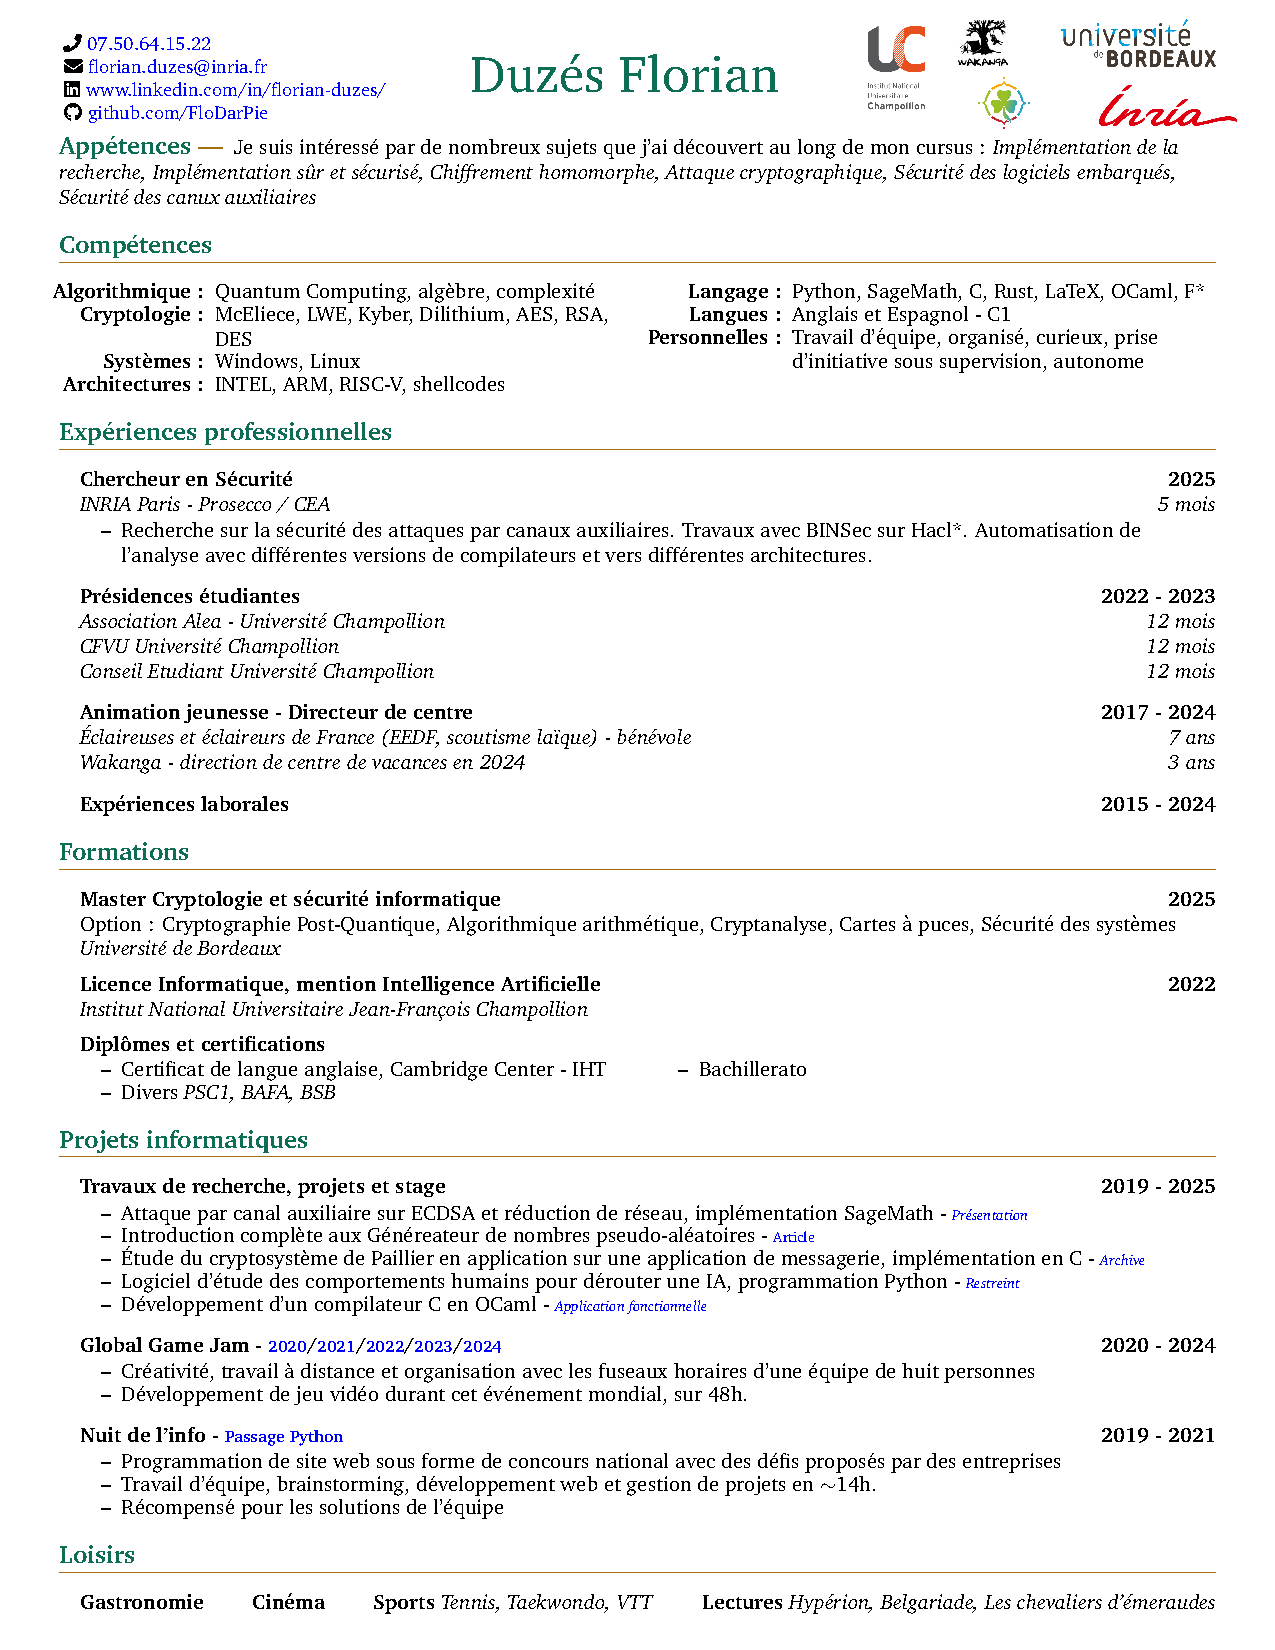
\includegraphics[scale=0.23]{imgs/DUZÉS_Florian.pdf}
    \end{column}
    \begin{column}{0.5\textwidth}
      \begin{block}{Mél}
        \footnotesize
        Je suis Florian Duzes. Je suis en train de terminer mon master en
        Cryptologie et Sécurité Informatique, à Bordeaux, avec un stage aux
        côtés de M. Aymeric Fromherz à l'INRIA Paris sur la sécurité de Hacl*
        face aux attaques par canaux auxiliaires par mesures de temps.

        Je voudrais poursuivre avec une thèse en lien avec mon sujet, mais je
        suis plus généralement intéressé par la programmation séurisée, la
        sécurité embarqué et la sécurité des systèmes face aux canaux
        auxiliaires.

        Mon cœur balance aussi vers la programmation cryptographique,
        l'implémentation de recherche en cryptologie, le chiffrement homomorphe
        et la cryptologie post-quantique.

        Je viens vous demander si vous connaissez une personne qui puisse être
        intéressée ou si vous connaissez quelqu'un qui puisse m'aiguiller pour
        trouver une thèse en lien avec ces sujets.
      \end{block}
    \end{column}
  \end{columns}
\end{frame}



%%--%%--%%--%%--%%--%%--%%--%%--%%--%%--%%--%%--%%--%%--%%
 
\section{Antoine geimer}
\frame{\sectionpage}

\begin{frame}{Courte présentation}
  \begin{columns}
    \begin{column}{0.6\textwidth}
      \begin{block}{Antoine Geimer}
        \begin{itemize}
          \item Thèsard à l'université de Lille
          \item Sujet : \textbf{Détection automatique de vulnérabilités dues aux canaux auxiliaires microarchitecturaux.}
          \item Intervention à l'INRIA le 16/06
          \item Dépôt Github de son article
        \end{itemize}
      \end{block}
    \end{column}
    \begin{column}{0.4\textwidth}
      \begin{center}
        \newlength{\imagewidth}
        \settowidth{\imagewidth}{\includegraphics{../../../../article/ccs23_geimer.pdf}}
        \includegraphics[trim = 0 0.5\imagewidth{} 0 0,clip,scale=0.3]{../../../../article/ccs23_geimer.pdf}
      \end{center}
    \end{column}
  \end{columns}
\end{frame}


%%--%%--%%--%%--%%--%%--%%--%%--%%--%%--%%--%%--%%--%%--%%



\section{Conclusion}
\frame{\sectionpage}

\begin{frame}{Conclusion}

  \begin{columns}
    \begin{column}{0.3\textwidth}
      \begin{block}{Un stage super intéressant}
        \begin{itemize}
          \item Riche
          \item Ouverture au monde
        \end{itemize}
      \end{block}
    \end{column}
    \pause
    \begin{column}{0.3\textwidth}
      \begin{block}{Modèle de travail}
        \begin{itemize}
          \item À reconcevoir
          \item À fixer les prochaines missions
        \end{itemize}
      \end{block}
    \end{column}
    \pause
    \begin{column}{0.3\textwidth}
      \begin{block}{Travaux à déterminer}
        \begin{itemize}
          \item \textit{\footnotesize Je note tous sur mon carnet}
        \end{itemize}
      \end{block}
    \end{column}
  \end{columns}

\end{frame}

%%%%%%%%%%%%%%%%%%%%%%%%%%%%%%%%%%%%%%%%%%%%%%%%%%%%%%%

%% Le texte est modifiable en changeant \thankyou
%% \renewcommand{\thankyou}{Thank You.}
\frame{\merci}


\end{document}

